\chapter{Modelo de Jaynes-Cummings}
\label{ch3_jcm}

%CAMBIAR ESTO PARA PERSONALIZARLO A MI GUSTO
\pagestyle{fancy}
\fancyhf{}
\fancyhead[LE]{\nouppercase{\rightmark\hfill}}
\fancyhead[RO]{\nouppercase{\leftmark\hfill}}
\fancyfoot[LE,RO]{\hfill\thepage\hfill}

En este capitulo analizaremos en profundidad la din\'amica y los aspectos teoricos mas importantes 
del modelo de Jaynes-Cummings, abordando el problema tanto desde un lado te\'orico, como desde
el lado computacional, necesario para resolver la din\'amica en sistemas abiertos.
Primero se trabajar\'a en el modelo de un átomo en una cavidad, se analizar\'an los casos importantes,
y se explicar\' la din\'amica del problema. Esto es importante para comprender conceptualmente como
interact\'uan fundamentalmente la materia y la luz, y nos sirve para conseguir buena intuici\'on del
problema de dos átomos. Tambien se ver\'a la influencia del entorno sobre la cavidad, permitiendo
perdida (o absorci\'on) de fotones, y tambien el bombeo coherente que puede excitar espontaneamente
al átomo. \newline

\section{Modelo y aproximaciónes}
Comencemos entonces por el paradigmatico modelo de 1 átomo. El modelo de Jaynes-Cummings consiste en describir la interacción entre la materia y la luz de manera cuantica, y el experimento mas sencillo consta de un átomo de dos niveles atrapada en una cavidad. La simpleza del modelo surge de las aproximaciónes e hipotesis que se hacen, en primer lugar, el campo electromagnetico dentro de la cavidad puede en principio tener infinitos modos, pero para simplificar se considera solo un modo. 
Entonces tenemos un Hamiltoniano ($\hbar = 1$)

\begin{equation}\label{eq3:hamiltoniano inicial}
\begin{aligned}
    \hat H & = \hat H_A + \hat H_C + \hat H_{int}  \\
    \hat H_A &= \omega \frac{\sigma_z}{2} \\
    \hat H_C &= \epsilon \hat a^\dagger\hat a = \epsilon \hat n \\
    \hat H_{int} &= -i g (\hat\sigma_-+\hat \sigma_+)(\hat a - \hat a^\dagger)
\end{aligned}
\end{equation}
donde $\epsilon$ y $\omega$ son las frecuencias naturales de la cavidad y del átomo respectivamente. Los operadores $\hat a$ y $\hat a^\dagger$ son los operadores de aniquilaci\'on y creaci\'on fot\'onicos de la cavidad y $\hat n =a^\dagger a$ es el operador de n\'umero de la cavidad, y $\hat \sigma_z$ es el operador de pauli. Los estados del átomo de dos niveles los llamamos $\ket{g}$ y $\ket{e}$ al estado ground y excitado respectivamente, y con esta notación los operadores $\sigma_\pm = (\sigma_x\pm i\sigma_y)/2$ son los operadores de subida y bajada atómicos. 
La interacci\'on es complicada, y para simplificar lo que se hace es usar la representaci\'on de interacci\'on, y uno encuentra que hay dos frecuencias, una que llamamos \textit{rotante} y es la diferencia entre las frecuencias características $\epsilon-\omega$, y la otra frecuencia es la suma $\epsilon+\omega$. La aproximación de onda rotante vale cuando las frecuencias son similares $\epsilon\sim\omega$, y consta de despreciar la dinámica de los términos contrarrotantes, ya que oscilan muy rápidamente en comparación con los términos rotantes, y entonces podemos promediar los efectos de los términos rápidos. Entonces al aplicar esta aproximación, justificada cuando $\epsilon\sim\omega$ y $g \ll \epsilon,\omega$ se obtiene el hamiltoniano de JC \ref{}\textcolor{red}{ludmi 49}
\begin{equation}
    H_{JC}=\epsilon a^\dagger a + \omega \sigma_z/2 + g(a^\dagger\sigma_-+a\sigma_+)
\end{equation} 
La interpretaci\'on de la interacci\'on en este caso es clara, las dos opciones son que el átomo suba un nivel de energ\'ia y en consecuencia la cavidad pierda un fot\'on, o que el átomo baje un nivel, y la cavidad gane una excitaci\'on. Este Hamiltoniano conserva el n\'umero total de excitaciones $\hat N= \hat n + \hat \sigma$. En este momento es usual aplicar una transformación unitaria $K=\exp{-i\omega t(a ^\dagger a + \sigma_z/2)}$ sobre el Hamiltoniano que queda 
\begin{equation}\label{eq3:hamiltoniano jcm}
    H=\frac{\Delta}{2}\sigma_z+g(a^\dagger \sigma_-+a \sigma_+)
\end{equation}
donde $\Delta = \epsilon - \omega$ es el \textit{detunning} entre las frecuencias de la cavidad y el átomo. Un ejemplo de esto es un átomo de Rydberg metido en una cavidad \ref{}, o ... \textcolor{red}{BUSCAR EJEMPLOS}.
Como el Hamiltoniano conserva la cantidad de excitaciones es oportuno agrupar los estados en funci\'on de la cantidad de excitaciones: $\{\ket{g,n},\ket{e,n-1}\}$. En esta base el Hamiltoniano se diagonaliza por bloques, ya que las interacciones conservan la cantidad total de excitaciones, entonces los elementos de matriz entre estados con diferente cantidad de excitaciones se corresponde
\begin{align*}
    [H,\hat N]=0 \implies & \bra{N'}H \hat N \ket{N} = \bra{N'}\hat N H \ket{N} \\
    & N \bra{N'}H  \ket{N} = N' \bra{N'}H \ket{N} \\
    & \implies \bra{N'}H \ket{N} = \begin{cases}
        0 \text{ , si } N' \neq N \\
        \bra{N}H \ket{N} \text{ , si } N'=N
    \end{cases}
\end{align*}
donde $\ket{N}$ es un estado con $N$ excitaciones totales. Entonces para resolver el problema solo tenemos que mirar el subespacio de 2x2 de n excitaciones, cuyo Hamiltoniano es
\begin{equation}
    H_n=\begin{pmatrix}
        -\frac{\Delta}{2} & g \sqrt{n} \\
        g \sqrt{n} & \frac{\Delta}{2} 
    \end{pmatrix}
\end{equation}
Resolvemos el problema de autovalores y autovectores y obtenemos
\begin{equation}
    \begin{aligned}
        \ket{\psi^n_-} & = \cos \frac{\theta_n}{2}\ket{g,n}-\sin \frac{\theta_n}{2}\ket{e,n-1} \\
        \ket{\psi^n_+} & = \sin \frac{\theta_n}{2}\ket{g,n}+\cos \frac{\theta_n}{2}\ket{e,n-1}        
    \end{aligned}
\end{equation}
con $E_{\pm}^n=\pm \frac{\Omega_n}{2}$ las autoenergias y $\Omega_n=\sqrt{\Delta^2+4g^2n}$ la frecuencia de Rabi del sistema, $\cos \theta_n=\frac{\Delta}{\Omega_n}$ modulando la superposici\'on de estados. 
\begin{figure}
    \centering
    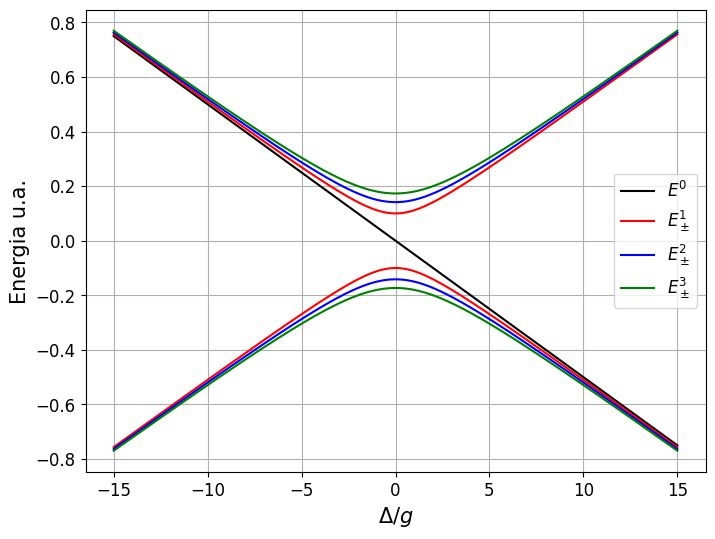
\includegraphics[width=0.7\textwidth]{figuras/ch3/relacion energia detunning jcm simple.png}
    \caption{Relaci\'on energ\'ia detunning para el modelo de Jaynes-Cummings. La diferencia de energ\'ia entre los estados de un mismo nivel para $\Delta=0$ es $2g\sqrt{n}$.}
    \label{fig:relación energia detunning jcm1}
\end{figure}
En la figura \ref{fig:relación energia detunning jcm1} se observan las curvas de energ\'ia en funci\'on del detunning para diferentes niveles. Lo primero que tenemos que observar es que en el caso resonante, es decir $\Delta=0$, los autoestados del sistema son los estados máximamente entrelazados de Bell
\begin{equation}
    \ket{\psi_\pm^n}=\frac{1}{\sqrt{2}}(\ket{gn}\pm\ket{e,n-1})
\end{equation} 
y la diferencia de energ\'ia entre los autoestados es $\Delta E^n =E^n_+-E^n_-=2g\sqrt{n}$. En el caso muy lejos de resonancia podemos asumir que $\Delta \gg g $, y entonces los autoestados coinciden en este l\'imite con los estados de la base, 
\begin{equation}
    \begin{aligned}
        \ket{\psi^n_+}=\ket{e,n-1} \\
        \ket{\psi^n_-}=\ket{g,n}
    \end{aligned}
\end{equation}
Ac\'a hay una sutileza, y es que si $\Delta>0$, entonces $\ket{e,n-1}$ es el estado de mayor energ\'ia y la notaci\'on coincide con la energ\'ia, pero si $\Delta<0$ entonces el estado $\ket{\psi^n_+}$ es el estado de menor energ\'ia. 
Un efecto interesante es que en el caso de alta desinton\'ia, podemos calcular la diferencia entre la energía del autoestado exacto del Hamiltoniano $\ket{\psi_\pm^n}$ y la energía asintótica a la que tiende, que es la energía de los estados de la base $\ket{g,n},\ket{e,n-1}$. Esta diferencia ... \textcolor{red}{VOLVER A ESTO Y VER SI DEJARLO O SACARLO. EVENTUALMENTE COMPLETAR.}
\begin{equation}
    \begin{aligned}
        \Delta E_{e,n-1}=E_+^n-E^{(0)}_{e,n-1}=\frac{g^2}{\Delta}n
        \Delta E_{g,n}=E_-^n-E^{(0)}_{g,n}=-\frac{g^2}{\Delta}n
    \end{aligned}
\end{equation}
El resultado importante de esta diferencia de energías es que aun en ausencia de fotones en la cavidad $n=0$, hay una diferencia entre las energías entre el Hamiltoniano del átomo, y del $H_{JC}$. Este efecto es el \textit{Lamb Shift} y nos dice que el vac\'io electromagnetico induce un corrimiento en la energ\'ia de los estados. Esto es importante notarlo, porque para el caso de dos átomos también est\'a manifiesto.

\subsection{Fase geométrica en el JCM}
Vamos a analizar la fase de Berry y la fase geométrica en la aproximación cinemática.
\subsubsection{Fase de Berry}
Para ver la fase de berry tenemos que tener un parámetro de control en el Hamiltoniano, el cual varía lentamente. Para esto necesitamos aplicar una transformación unitaria de corrimiento de fase al Hamiltoniano original \ref{eq3:hamiltoniano jcm} $R=\exp{-i\Omega a^\dagger a}$, que queda
\begin{equation}
    H=\frac{\Delta}{2}\sigma_z+g(a^\dagger \sigma_e^{-i\Omega}-+a\sigma_+e^{i\Omega})
\end{equation}
que ahora depende explicitamente del parámetro externo de control $\Omega$. Los autoestados de este nuevo Hamiltoniano se obtienen aplicando esta misma transformación sobre los autoestados del Hamiltoniano original. Si el parámetro de control varia lentamente entre 0 y $2\pi$, entonces estamos dentro de las hipótesis propuestas por Berry, y podemos calcular la fase de Berry mediante la ecuación \ref{eq2:fg berry}:
\begin{equation}
    \psi_a^n=i\oint_Cd\Omega\bra{\psi_\pm^n}R(\Omega)^\dagger \frac{d}{d\Omega}\ket{\psi_\pm^n}=\pi(1\pm \cos(\theta_n))
\end{equation}

que es no trivial incluso para $n=0$, lo que nos dice que incluso el vacío electromagnetico introduce una corrección en la fase de Berry.
\subsubsection{Aproximación Cinemática}
Para comparar ambos métodos, ahora vamos a calcular la fase geométrica utilizando la aproximación cinemática aunque este abordaje es más general de lo necesario en este caso.
Si se considera que el estado inicial es un atuoestado del Hamiltoniano, como los estados $\ket{\psi_\pm^n}$, entonces la fase geométrica en este caso se anula. Pero si se considera un estado inicial, por ejemplo $\ket{\psi(0)}=\ket{e,n}$, entonces el estado a tiempo $t$ resulta
\begin{equation}\label{eq3:fg berry jcm}
    \ket{\psi(t)}=(\cos^2\theta_ne^{-iE_+^nt}+\sin^2\theta_ne^{iE_+^nt})\ket{e,n}-i \sin\theta_n\sin(E_+^nt)\ket{g,n+1}
\end{equation}
La fase geométrica acumulada \ref{eq2:fg cinematica unitaria} es
\begin{equation}\label{eq3:fg unitaria jcm}
    \phi_u[C]=-\pi(1-\cos\theta_n)\frac{t}{T} +\arg\left\{ 1+e^{2\pi i \frac{t}{T}}\frac{\Omega_n-\Delta}{\Omega_n+\Delta} \right\}
\end{equation}
con $T=\frac{2\pi}{\Omega_n}$ es un período correspondiente a la frecuencia de Rabi $\Omega_n$. Esta expresión y la anterior \ref{eq3:fg berry jcm}, deberían coincidir cuando $t=T$, que se corresponde con un ciclo cerrado. En este caso ($t=T$) se obtiene
\begin{equation}
    \phi_u=-\pi(1-\cos\theta_n)
\end{equation}
La diferencia de signos se puede explicar comparando las curvas descritas por la esfera de Bloch para cada evolución. 
\begin{figure}[H]
    \centering
    \begin{subfigure}[h]{0.49\textwidth}
        \centering
        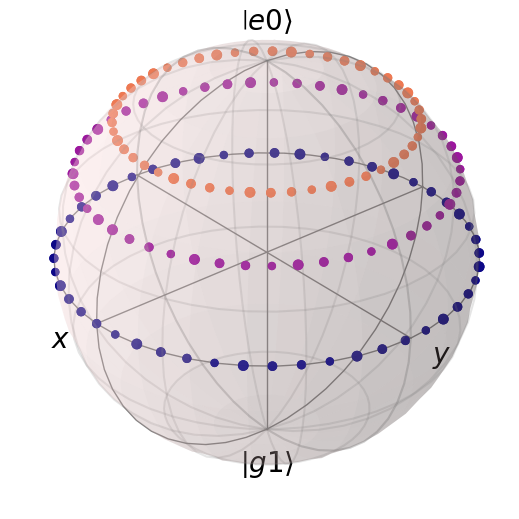
\includegraphics[width=\textwidth]{figuras/ch3/bloch berry.png}
        \caption{Evolución adiabática} 
        \label{fig3:bloch berry}
    \end{subfigure}
    \hfill
    \begin{subfigure}[h]{0.49\textwidth}
        \centering
        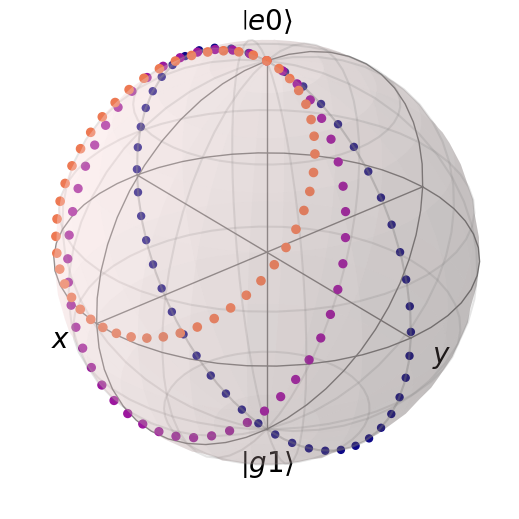
\includegraphics[width=\textwidth]{figuras/ch3/bloch cinematica.png}
        \caption{Enfoque cinemático}
        \label{fig3:bloch cinematica}
    \end{subfigure}
    \caption{}
    \label{fig3:esfera de bloch jcm}
\end{figure}
En el caso \ref{eq3:fg berry jcm}, correspondiente a la figura \ref{fig3:bloch berry}, los autoestados son los autoestados $R(\Omega)\ket{\psi_\pm^n}=e^{-i\Omega \hat n}\ket{\psi_\pm^n}$, entonces al variar $\Omega\in [0,2\pi]$ la trayectoria es simplemente un circulo en la esfera de Bloch. En cambio, en el segundo caso, si preparamos el sistema inicialmente en el estado $\ket{e,n}$ y lo dejamos evolucionar por la acción de H durante un tiempo, la trayectoria ahora no son círculos horizontales en la esfera, sino que parten del polo norte, que es el estado $\ket{e,n}$, y luego hace una trayectoria ovalada, para finalmente volver al punto inicial de partida a un tiempo $t=T$. La diferencia en el signo se explica a través de la transformación que nos lleva de una curva a la otra. Para esto, necesitamos de una rotación rígida, y una inversión de la parametrización, por su parte, esta ultima, introduce un signo negativo, cosa que se ve claramente en la ecuación \ref{eq3:fg unitaria jcm} al cambiar $t\rightarrow -t$.

\section{Medio Kerr}\label{sec3:medio kerr}
Ahora que ya se trabajó el caso mas sencillo, se comienza a estudiar casos mas generales. La primera generalización que se hará es agregar un medio no lineal. Este medio se lo conoce como medio Kerr, y lo que hace es agregar un término en el Hamiltoniano de la cavidad, que pasa de ser \ref{eq3:hamiltoniano inicial} 
\begin{equation}
    H_C=\epsilon \hat n \rightarrow H_C^{\text{Kerr}}=\epsilon \hat n (1-\frac{\chi}{\epsilon})
\end{equation}
donde $\chi$ es el parámetro que caracteriza al medio de la cavidad Kerr. Si se realizan nuevamente los mismos pasos, se arriba a las mismas conclusiones sobre la forma del Hamiltoniano, y se tiene que 
\begin{equation}
    H=\frac{\Delta}{2}\hat \sigma_z+\chi \hat n^2+g(\hat a^\dagger \hat \sigma_-\hat a \hat \sigma_+)
\end{equation}
y en forma matricial, en el subespacio de n excitaciones $\{\ket{gn},\ket{e,n-1}\}$
\begin{equation}
    H^{(n)} = \begin{pmatrix}
        -\frac{\Delta}{2}+\chi n^2 & g \sqrt{n} \\
        g \sqrt{n} & \frac{\Delta}{2}+\chi (n-1)^2 
    \end{pmatrix}
\end{equation}
Resolviendo, se obtiene que ahora los autovectores son
\begin{equation}
    \ket{\psi_\pm^n}=\frac{1}{N_\pm} \left( (-\frac{\Delta}{2}+\chi(n-1/2)\mp\frac{\Omega_{n,\chi}}{2}) \ket{gn} + g\sqrt{n} \ket{e,n-1}  \right)
\end{equation}
donde $\Omega_{n,\chi}=\sqrt{(\chi(n-1/2)-\Delta)^2+4g^2n}$, $N_\pm=\sqrt{(-\frac{\Delta}{2}+\chi(n-1/2)\mp\Omega_{n,\chi}/2)^2+g^2n}$, y las autoenergias son 
\begin{equation}\label{eq3:autoenergia kerr}
    E_\pm^n=\chi(n-\frac{1}{2})^2 +\frac{\chi}{4} \pm \frac{\Omega_{n,\chi}}{2}
\end{equation}
Se puede ver que el resultado con $\chi=0$ se reduce al caso visto anteriormente, que representa una cavidad con un medio lineal.

Si uno quiere resolver la dinámica de este problema para un estado inicial cualquiera, lo que tenemos que hacer es desarrollar este estado inicial en función de los autoestados del problema, entonces tendríamos para un estado arbitrario con un numero total de excitaciones definido, que suponemos igual a 1 por simplificación (la generalización es inmediata):
\begin{equation}
    \ket{\psi}(t)=U(t)(\braket{\psi_+^1}{\psi(0)}\ket{\psi_+^1}+\braket{\psi_-^1}{\psi(0)}\ket{\psi_-^1})=c_+e^{-iE_+t}\ket{\psi_+}+c_-e^{-iE_-t}\ket{\psi_-}
\end{equation}
Lo interesante de esto es que podemos sacar de factor común alguna de las dos energías, y entonces lo importante para la evolución temporal del sistema es la diferencia entre las energías, por lo tanto, la cantidad relevante sigue siendo $\Omega_{n,\chi}$, que es la frecuencia de Rabi para medios tipo Kerr. Por otro lado, el producto interno que da lugar a los coeficientes $c_\pm$ depende de $\chi$, por lo tanto las amplitudes de probabilidad de encontrar al estado temporalmente evolucionado en algún otro estado haciendo una medición proyectiva, depende de $\chi$. Por lo tanto, se puede decir que el medio Kerr modifica las amplitudes de oscilación de las poblaciones del estado.

Entonces se analiza la relación entre $\pm \Omega_{n,\chi}/2$ y el detunning, teniendo en cuenta que ahora el medio puede tener $\chi \neq 0$. 

\begin{figure}[H]
    \centering
    \begin{subfigure}[h]{0.49\textwidth}
        \centering
        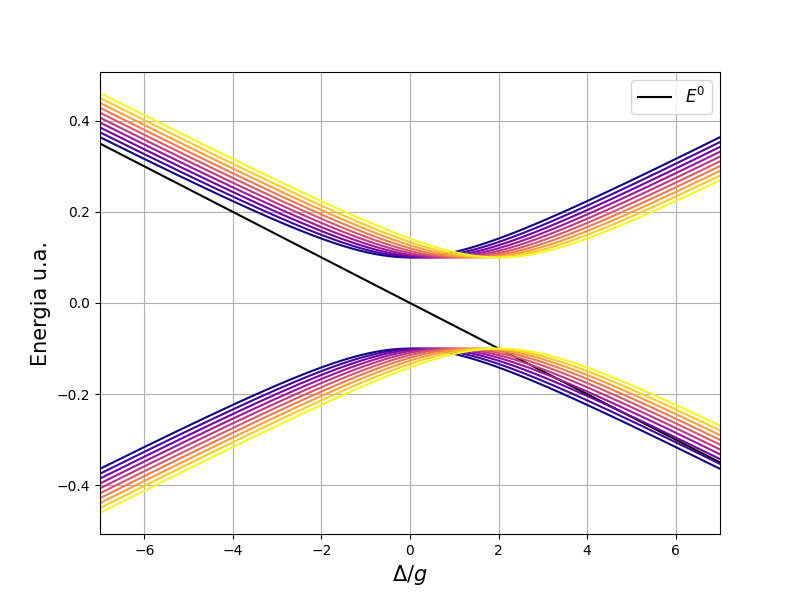
\includegraphics[width=\textwidth]{figuras/ch3/relacion energia detunning jcm simple kerr.png}
        \caption{N=1}
        \label{fig3:relacion energia detunning kerr 1}
    \end{subfigure}
    \hfill
    \begin{subfigure}[h]{0.49\textwidth}
        \centering
        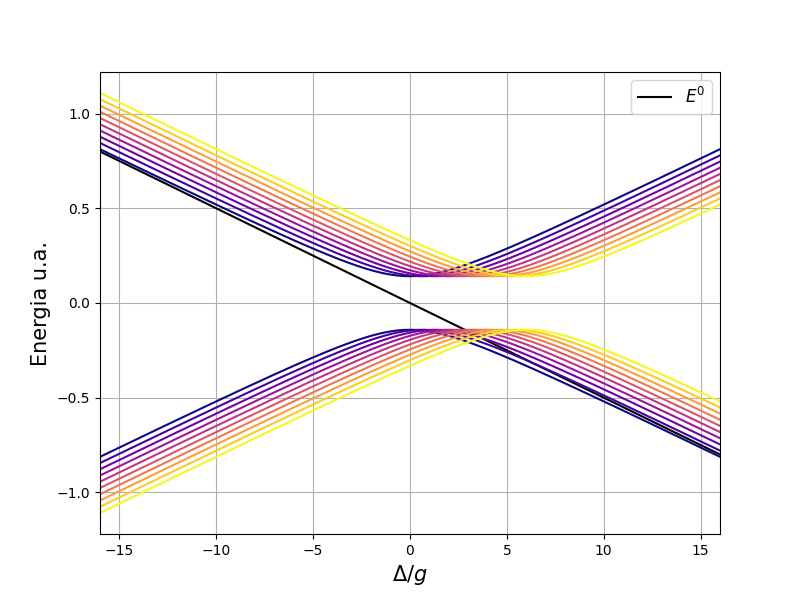
\includegraphics[width=\textwidth]{figuras/ch3/relacion energia detunning jcm simple kerr 2.png}
        \caption{N=2}
        \label{fig3:relacion energia detunning kerr 2}
    \end{subfigure}
    \caption{Grafico de la frecuencia de Rabi $\Omega_{N,\chi}$ en funcion del detunning $\Delta$ para N=1 y N=2.}
    \label{fig3:relacion energia detunning kerr}
\end{figure}

Se observa en la figura \ref{fig3:relacion energia detunning kerr} las diferencias entre autoenergias van cambiando para diferentes valores de $\chi$, donde en el panel \ref{fig3:relacion energia detunning kerr 1} se observa las energías para N=1 y en \ref{fig3:relacion energia detunning kerr 2} para N=3, en función del detunning, y en colores se ve de mas oscuro a mas claro, como el aumento de $\chi \in [0,2g]$ afecta a las curvas. Lo que se observa es que, al aumentar $\chi$, las curvas se desplazan hacia la derecha en una cantidad $\chi(n-1/2)$. 

Este comportamiento se puede predecir mirando la forma de la autoenergia \ref{eq3:autoenergia kerr}, ya que lo que estamos haciendo es desplazando la raiz haciendo un cambio de variables $\Delta \rightarrow \Delta - \chi(n-1/2)$. Este desplazamiento depende del número de excitaciones N. 
Dados dos valores diferentes de $\chi$ nos interesa saber si al aumentar $\Delta$, aumenta o disminuye las energías de los estados, para esto buscamos la intersección entre dos curvas con diferentes $\chi$, que llamamos $\chi_1$ y $\chi_2$, con $\chi_1<\chi_2$. Haciendo el calculo obtenemos que la intersección es para $\Delta=(2n-1)\frac{\chi_1+\chi_2}{2}$, es decir, si $\Delta<(2n-1)\frac{\chi_1+\chi_2}{2}$ entonces la frecuencia de $\chi_2$ es mayor que la de $\chi_1$ y por lo tanto oscila mas rápidamente, y viceversa si $\Delta>(2n-1)\frac{\chi_1+\chi_2}{2}$.

Ahora, habiendo entendido esto, podemos ver que el efecto del medio es modificar la frecuencia y también la amplitud de la oscilación, haciendo que la primera sea menor, y \textcolor{red}{para ver que pasa con las amplitudes tengo que hacer algunas cuentas}


\section{JCM disipativo}


Habiendo desarrollado el análisis de la fase geométrica acumulada por el sistema átomo-cavidad en la situación ideal de completo aislamiento, se aborda ahora el estudio para el escenario más realista en el que el mismo sistema se encuentra en interacción con un entorno. El problema se trata para la implementación específica en estructuras semiconductoras, en las que un punto cuántico (al cual se sigue, sin embargo, refiriendo como átomo o sistema de dos niveles) se ubica en una nano o micro-cavidad.

Siguiendo \cite{80}, en este capítulo se estudia en detalle la fase geométrica acumulada en un modelo de Jaynes-Cummings disipativo, como caso paradigmático dentro del campo de la electrodinámica en cavidades. Se considera que los principales mecanismos por los cuales el sistema “átomo + modo” interactúa con el entorno son el flujo de fotones a través de las paredes de la cavidad y el continuo e incoherente bombeo del sistema de dos niveles, lo que conforma un escenario frecuente en electrodinámica de cavidades semiconductoras \cite{81,82,83}. 

Para poder modelar estos mecanismos, se emplea la ecuación maestra fenomenológica de Lindblad
\begin{equation}\label{eq3:lindblad}
\dot{\rho}(t) = -i [H, \rho(t)] + \frac{1}{2} \sum_\alpha \big( 2L_\alpha \rho(t) L_\alpha^{\dagger} - \{ L_\alpha^{\dagger}L_\alpha, \rho(t) \} \big),
\end{equation}

, despreciando otros procesos con menor influencia en la dinámica como el desfasaje puro o el bombeo de fotones del entorno en la cavidad, considerando además que el entorno se halla a temperatura cero. Los operadores de Lindblad

\begin{equation}
L_\gamma = \sqrt{\gamma} \ a
\end{equation}
\begin{equation}
L_p = \sqrt{p} \ \sigma_+
\end{equation}

,representan la pérdida de fotones y el bombeo continuo e incoherente del átomo, respectivamente, con los parámetros $\gamma$ y $p$ denominados tasa de pérdida de fotones y amplitud del bombeo. 

El bombeo sobre el átomo es siempre secundario frente a la pérdida de fotones, lo cual nos da las relaciones $\frac{p}{g},\frac{p}{\gamma} \ll 1$, y la relación entre $\gamma$ y $g$ da lugar a dos regímenes que se diferencian con claridad \cite{50}-\cite{54}. El régimen de acoplamiento fuerte (SC o Strong Coupling) es cuando la interacción átomo-cavidad es mas fuerte que la disipación del entorno, es decir $\gamma /g <1$. En el caso contrario $\gamma/g>1$ estamos en el régimen de acoplamiento débil (WC o Weak Coupling). Para no generar confusiones, hay que destacar que en general, cuando en la literatura se habla de acoplamientos fuertes y débiles, se refiere a la interacción entre las partes del mismo sistema, pero en este caso, se esta haciendo referencia a la interacción del sistema con el entorno EN COMPARACIÓN con la interacción interna del sistema.

En esta ocasión nos interesa resolver el problema restringiendonos al subespacio donde el átomo puede estar en cualquiera de sus dos estados, y nos restringimos al caso en donde la cavidad tiene 1 o 2 fotones, en consecuencia, se restringe el estudio a un subespacio truncado cuya base son los estados $\{ \ket{0}=\ket{g,0} ; \ket{1}=\ket{e,0} ; \ket{2}=\ket{-,1} \}$. Desarrollando explícitamente el sistema de ecuaciones dadas por la ecuación de Lindblad \ref{eq3:lindblad}, obtenemos que los elementos $\rho_{0i}$ quedan desacoplados de los demás:

\begin{equation}
    \begin{aligned}
        \dot \rho_{01} & =-\frac{p}{2} \rho_{01}+i\Delta\rho_{01}+ig\rho_{02} \\
        \dot \rho_{02} & =-\frac{p}{2} \rho_{02}-\gamma \rho_{02}+ig\rho_{01}
    \end{aligned}
\end{equation}

,con lo cual, si inicialmente los elementos de matriz $\rho_{0i}(0)=0$, permanecerán así durante toda la evolución del sistema. Para hacer una analogía y realizar una comparación con el caso unitario, se estudia la condición inicial $\rho(0)=\ketbra{e,0}{e,0}$, que satisface esta condición, de manera que se espera que el estado $\rho(t)$ exciba una estructura diagonal por bloques. El primer bloque de 1x1 representando al estado $\ket{0}$, y luego un bloque de 2x2 que describe la dinámica entre los estados $\ket{1}$ y $\ket{2}$. Las ecuaciones son

\begin{equation}
\begin{aligned}
\dot{\rho}_{00} &= -p \rho_{00} + \gamma \rho_{22}, \\
\dot{\rho}_{11} &= -i g (\rho_{21} - \rho_{12}) + p \rho_{00}, \\
\dot{\rho}_{22} &= -i g (\rho_{12} - \rho_{21}) - \gamma \rho_{22}, \\
\dot{\rho}_{12} &= -i g (\rho_{22} - \rho_{11}) - i \Delta \rho_{12} - \frac{\gamma}{2} \rho_{12}.
\end{aligned}
\end{equation}

que se resuelven numéricamente para acceder al estado $\rho(t)$ a tiempo $t>0$. 

\begin{figure}[H]
    \centering
    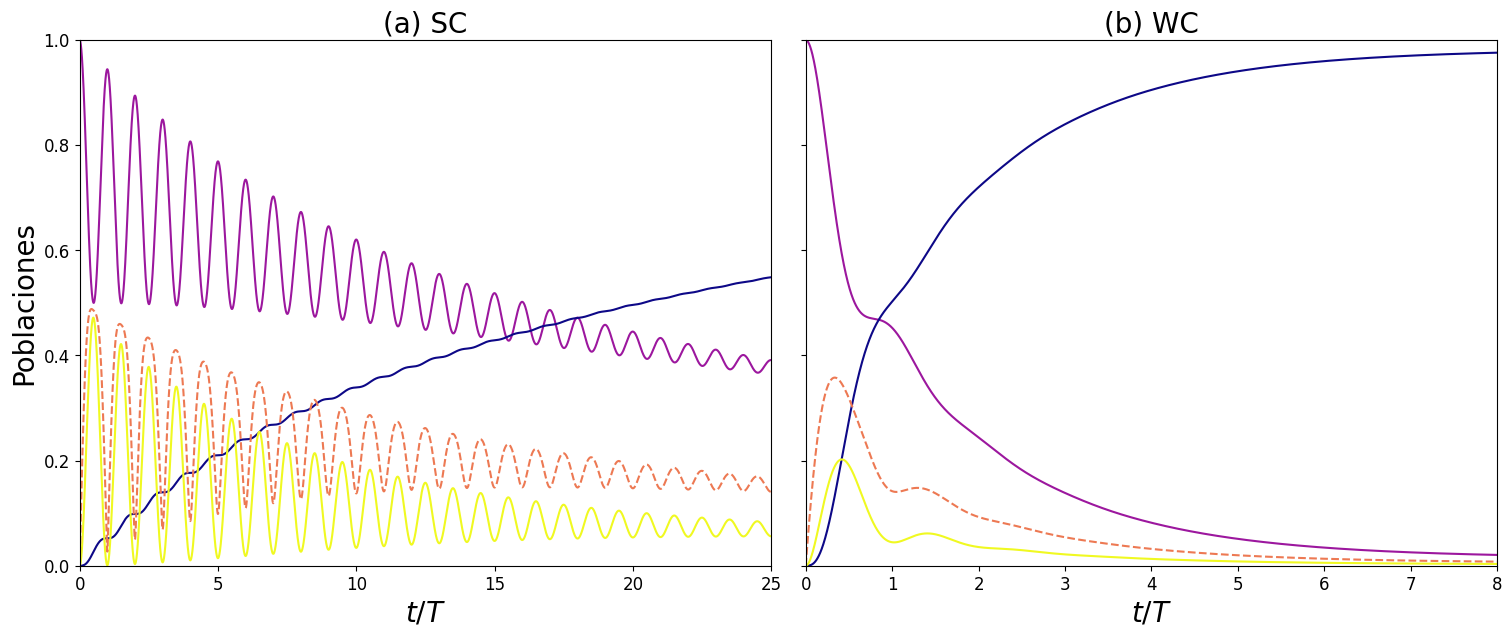
\includegraphics[width=\textwidth]{figuras/ch3/poblaciones sc vs wc.png}
    \caption{Solución numérica al sistema de ecuaciones dada por la ecuación de Lindblad para el estado inicial $\ket{e0}\bra{e0}$. Estos gráficos se realizaron con $\Delta=2g$; a la izquierda se observa el regimiento de Weak Coupling con $\gamma=0.1g$, donde el sistema átomo-cavidad esta débilmente acoplado con el entorno, y a la derecha el de Strong Coupling con $\gamma=2g$, donde las poblaciones y coherencias decaen sin oscilar. Las lineas solidas son las poblaciones de los estados, en azul para el estado $\ket{g0}$, en morado para $\ket{e0}$ y en amarillo $\ket{g1}$, y la linea rayada representa la coherencia entre los estados con N=1 ($\ket{e0}$ y $\ket{g1}$). }
    \label{fig3:poblaciones e0}
\end{figure}

En el panel \ref{fig3:poblaciones e0}a, se muestra el régimen de SC, donde el acoplamiento entre el átomo y la cavidad es mayor al acoplamiento con el entorno, según la relación entre los parámetros $\gamma/g=0.1$, y en el panel \ref{fig3:poblaciones e0}b, se muestra el caso del WK. La diferencia que es interesante para el problema, es que en el primer caso, tanto las poblaciones como las coherencias presentan oscilaciones coherentes antes de decaer por la influencia del entorno. En cambio, para el caso de WK, estas oscilaciones coherentes no están presentes y el sistema llega a su estado asintótico en tiempos muy cortos. Las características de la dinámica de cada régimen, influyen profundamente en el estudio de la fase geométrica, haciendo posible unicamente su utilización en el caso de Strong Coupling, donde la dinámica presenta oscilaciones coherentes durante varios ciclos, antes de decaer, haciendo del régimen de SC el único escenario conveniente para su estudio. Antes de fundamentar esta afirmación, se realiza un estudio poblacional en el caso de una cavidad con medio Kerr.

Como se vio anteriormente, el efecto del medio Kerr sobre los autoestados y las autoenergias es, por un lado, desplazar los niveles de energía.
\begin{figure}
    \centering
    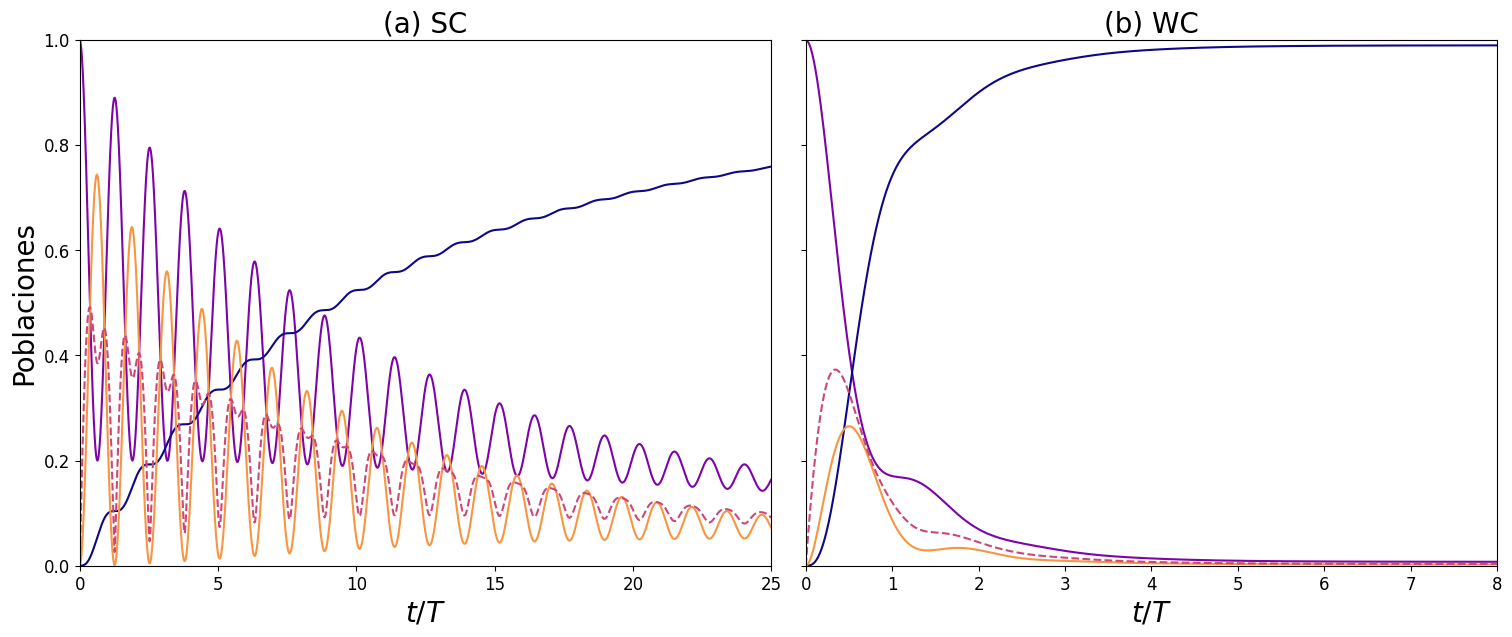
\includegraphics[width=\textwidth]{figuras/ch3/poblaciones kerr.png}
    \caption{Análisis poblacional para una cavidad con medio Kerr con $\chi=0.5g$.}
    \label{fig3:poblaciones kerr}
\end{figure}
Si se comparan las figuras \ref{fig3:poblaciones e0} con \ref{fig3:poblaciones kerr}, entonces se pueden observar dos diferencias. La primera es lo mencionado anteriormente; en el mismo tiempo, es decir entre $0\leq t/T \leq 25$, en el caso de $\chi=0$ se observan 25 oscilaciones, pero en el caso de $\chi=0.5g$ solo se observan 23 oscilaciones. Esto se debe a la condición que se encontró al final de la sección \ref{sec3:medio kerr}, en este caso se cumple que $\Delta=2g>(2n-1)\frac{\chi_1+\chi_2}{2}=1\cdot\frac{0.5g}{2}$, entonces la diferencia de energías entre los autoestados disminuye al aumentar $\chi$, y por lo tanto las oscilaciones son mas lentas para el caso de $\chi=0.5g$ en comparación con $\chi=0$.

\subsection{Fase geométrica en presencia de disipación}
Ahora se estudia la fase geométrica adquirida por el sistema, calculada siguiendo la definición \ref{}, y como esta se ve modificada con respecto del valor unitario por efecto del contacto con el entorno. Como el estado inicial es puro, la definición se reduce al caso particular descrito por la ecuación \ref{eq2}.

Los autovalores y autovectores del operador densidad pueden escribirse formalmente  diagonalizando el subespacio de 2x2 de la matriz densidad:
\begin{equation}
    \rho(t)=\begin{pmatrix}
        \rho_{00} & 0 & 0 & 0 &\dots \\
        0 & \rho_{11} & \rho_{12} & 0 & \dots \\
        0 & \rho_{21} & \rho_{22} & 0 & \dots \\ 
        \vdots & 0 & 0 & \ddots & \dots 
    \end{pmatrix}
\end{equation}
donde estamos nuevamente asumiendo una estructura diagonal por bloques, que se da cuando el estado inicial tiene un numero definido de excitaciones, dando lugar a dos autovectores. El de interés para utilizar la definición de la fase geométrica \ref{}, es el autoestado
\begin{equation}
    \ket{\psi_+}(t)=\frac{-(\rho_{22}-\epsilon_+)\ket{e,0}+\rho_{21}\ket{g,1}}{\left((\rho_{22}-\epsilon_+)^2+\rho_{21}\rho_{12} \right)^{1/2}}
\end{equation}
con $\epsilon_+=\frac{1}{2}(\rho_{11}+\rho_{22}+((\rho_{11}-\rho_{22})^2+4\rho_{12}\rho_{21})^{1/2})$ el autovalor asociado. Recurriendo a este resultado, podemos escribir formalmente la fase geométrica en función de los elementos de matriz $\rho_{ij}(t)$:
\begin{equation}
    \phi_g(t)=\int_0^t dt' \frac{\Im \dot\rho_{21}\rho_{12}}{(\rho_{22}-\epsilon_+)^2+\rho_{12}\rho_{21}}
\end{equation}

En general, esta fase diferirá de aquella acumulada en una evolución unitaria de forma que puede
escribirse, sin pérdida de generalidad, $\phi_g=\phi_u+\delta\phi$, con $\delta\phi$ la diferencia entre la fase unitaria y
aquella modificada por la presencia del entorno. Caracterizar la corrección $\delta\phi$ permite relacionar este
objeto, perteneciente a la geometría misma del espacio de Hilbert, con los efectos de disipación y
decoherencia experimentados por el sistema, así como determinar bajo qué circunstancias $\delta\phi$ resulta
despreciable y se puede considerar que la fase geométrica es robusta al efecto del entorno.

\subsubsection{Dependencia con el régimen de acoplamiento}
En la figura \ref{fig3:fg gamma} se muestra la fase geométrica acumulada en función del tiempo, para el estado inicial puro $\ket{e,0}$, comparando 4 casos para la relación $\gamma|g$ pertenecientes al régimen de SC, ademas como referencia se muestra la fase geométrica unitaria.
\begin{figure}[H]
    \begin{minipage}[c]{0.67\textwidth}
        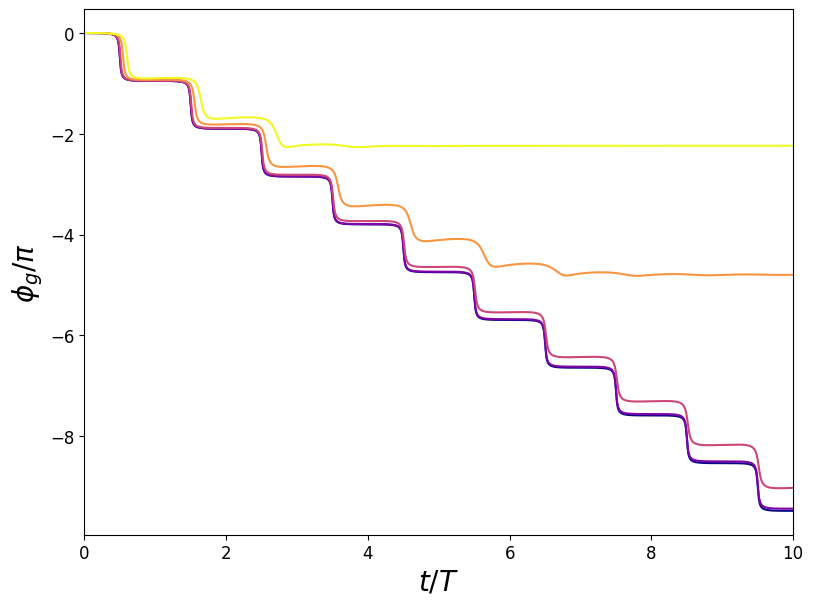
\includegraphics[width=\textwidth]{figuras/ch3/fg gamma.png}
      \end{minipage}\hfill
      \begin{minipage}[c]{0.3\textwidth}
        \caption{
            Fase geométrica acumulada por un sistema con un detunning $\Delta=0.1g$, para diferentes valores característicos del entorno. En todos los casos la tasa de bombeo es $p=0.005g$, y se muestran diferentes valores para $\gamma$, partiendo de $\gamma=0$ perteneciente a la linea azul oscuro que es el caso unitario, y para $\gamma=0.01g$,$\gamma=0.1g$,$\gamma=0.5g$ y $\gamma=g$, correspondientes a las lineas violeta, rosa, naranja y amarilla.
        } \label{fig3:fg gamma}
      \end{minipage}
\end{figure}
Al aumentar la interacción con el entrono, aumenta la diferencia $\delta \phi$ entre la fase acumulada con aquella correspondiente al caso unitario. Sin embargo, si el valor aumenta demasiado, la perdida de coherencia detiene el movimiento del estado y consecuentemente la acumulación de fase. Por esto es que el estudio sobre la fase geométrica debe ser en el régimen de SC, ya que si la relación $\gamma|g\gg 1$, la fase dejara de acumularse luego de un periodo muy corto de tiempo.


\subsubsection{Dependencia con el detunning}
Ya que las amplitudes de los estados y las frecuencias de oscilación dependen de los parámetros del problema, entonces la curva que describe el estado en el espacio de rayos dependerá también de estos, heredando así la fase geométrica una dependencia con los parámetros. Manteniendo las características del entorno iguales, se estudia la dependencia de la fase geométrica con el detunning $\Delta$. En la figura \ref{fig3:fg detunning} se observa que conforme se aumenta el detunning átomo-cavidad, la fase acumulada es menor (en valor absoluto) y se suaviza.
\begin{figure}[H]
    \begin{minipage}[c]{0.67\textwidth}
        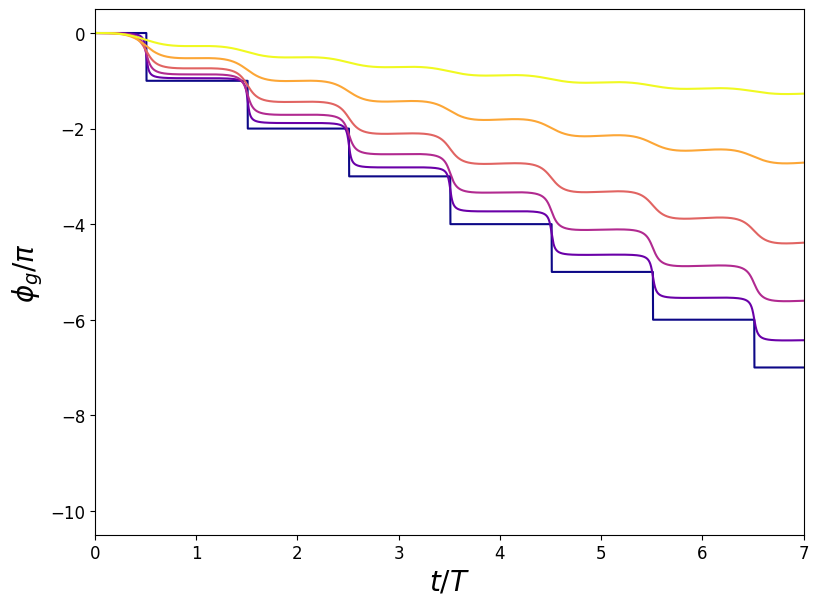
\includegraphics[width=\textwidth]{figuras/ch3/fg detunning.png}
    \end{minipage}\hfill
    \begin{minipage}[c]{0.3\textwidth}
    \caption{
         } \label{fig3:fg detunning}
  \end{minipage}
\end{figure}

Como se discutió anteriormente, la fase geométrica en presencia del entorno se puede descomponer en la parte unitaria $\phi_u$ dada por la ecuación \ref{ec2:}, más una corrección $\delta\phi$ que refleja la desviación introducida por el entorno. La dependencia de la componente unitaria en $\Delta/g$ esta explicita en la ecuación \ref{ec} ludmi eq 3.8, surge entonces la pregunta de la dependencia del termino $\delta\phi$ con respecto a los parámetros del problema, o si toda la dependencia se encuentra contenida en la parte unitaria $\phi_u$. Para tratar con esta pregunta se analiza la corrección $\delta\phi$ en un instante dado (que se elije y se mantiene fijo), observándola como función del valor de $\Delta/g$. El resultado se presenta en la figura \ref{fig3:deltaphi 0}, en el cual se contrasta ademas esta dependencia para tres entornos caracterizados por distintos valores de tasa de perdida de fotones $\gamma$.
\begin{figure}[H]
    \begin{minipage}[c]{0.67\textwidth}
        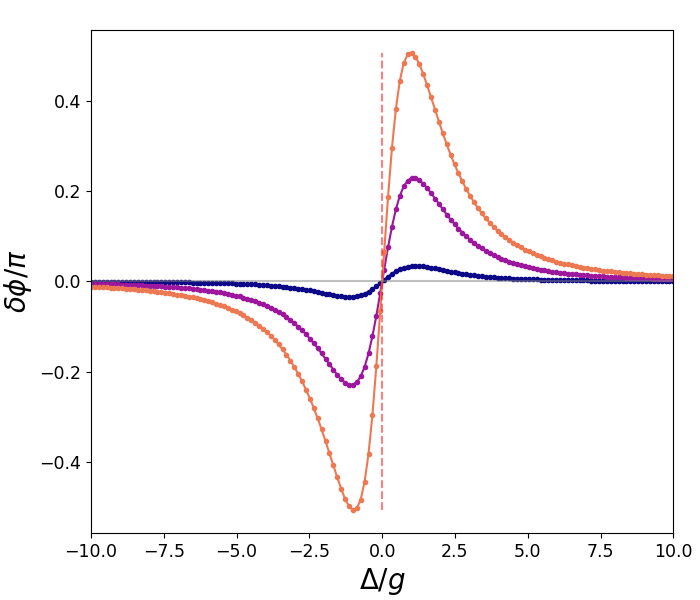
\includegraphics[width=\textwidth]{figuras/ch3/robustez.png}
    \end{minipage}\hfill
    \begin{minipage}[c]{0.3\textwidth}
    \caption{Diferencia de fase geométrica acumulada en función del detunning átomo-cavidad $\Delta$, para $\chi=0$ y para 3 medios distintos, cuyas tasas de perdida de fotones son $\gamma/g=0.01g,0.1g,0.25g$, asignadas a los colores violeta oscuro, morado y amarillo respectivamente.
         } \label{fig3:robustez 0}
  \end{minipage}
\end{figure}
Puede verse que la corrección en efecto depende del valor del detunning $\Delta/g$, y dos aspectos resaltan. En primer lugar es que la corrección se anula, en todos los casos considerados, cuando se satisface la condición de resonancia $\Delta=0$. Este hecho resulta prometedor,  insinuando que en este caso la fase geométrica $\phi_g$ resultaría robusta a los efectos de un entorno en el régimen de SC. La otra característica de la corrección $\delta\phi$ que se revela en la figura \ref{fig3:robustez 0} es la no-monotonicidad de la corrección como función de $\Delta/g$, que exhibe un extremo para un valor $\Delta/g$ que depende débilmente tanto en las constantes $\gamma/g$ y $p/g$ que caracterizan el entorno como en el instante $t$ en el que se realiza la observación. De esta forma la figura \ref{fig3:robustez 0} despierta un interés es doble, ya que permite identificar: (i) las condiciones en las cuales el efecto del entorno sobre la fase geométrica es mayor, acercando la posibilidad de una detección experimental y, (ii) las condiciones que mitigan, permitiendo ignorarlo, este efecto o incluso que lo eliminan por completo.

\subsubsection{Dependencia con el medio Kerr}

Ahora se considera la dependencia con el medio Kerr. Al estudiar los efectos del detunning, se considero que la cavidad era lineal, es decir $\chi=0$. Es el objeto de estudio de esta sección ver como se modifican la fase geométrica y los resultados obtenidos para el detunning al considerar un medio Kerr. En primer lugar, se muestra la dependencia de la fase geométrica acumulada para diferentes valores de $\chi/g$, considerando un entorno idéntico en todos los casos, y también considerando un valor fijo del detunning.

\begin{figure}[H]
    \centering
    \begin{subfigure}{0.49\textwidth}
        \centering
        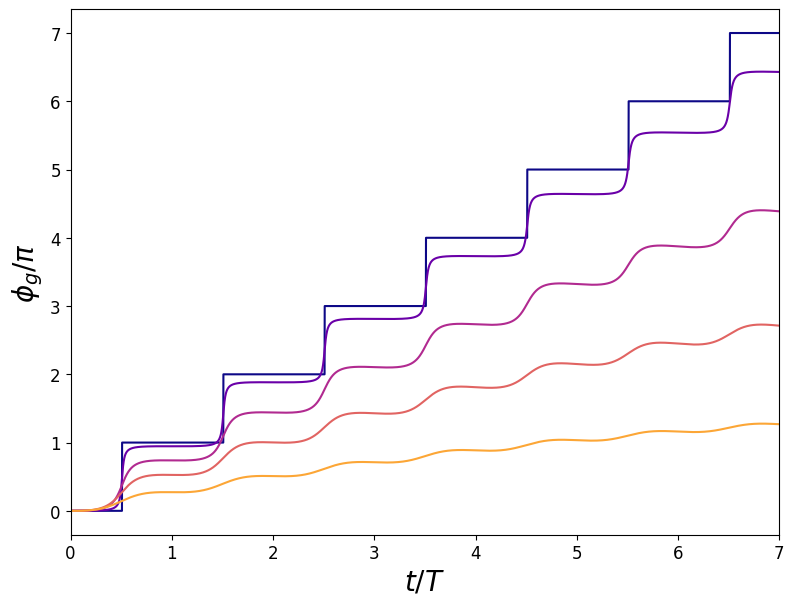
\includegraphics[width=\textwidth]{figuras/ch3/fg kerr.png}
        \caption{$\Delta=0$}
        \label{fig3:fg kerr 1}
    \end{subfigure}
    \hfill
    \begin{subfigure}{0.49\textwidth}
        \centering
        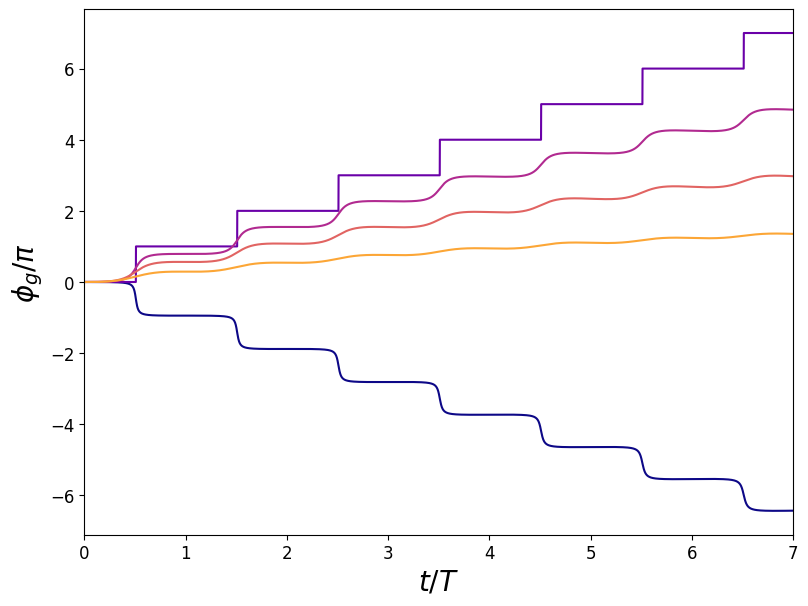
\includegraphics[width=\textwidth]{figuras/ch3/fg kerr d=0.1g.png}
        \caption{$\Delta=0.1g$}
        \label{fig3:fg kerr 2}
    \end{subfigure}
    \caption{}
\end{figure}
En el panel \ref{fig3:fg kerr 1} se observa el efecto del medio sobre la fase geométrica acumulada, donde se observa que la linea azul oscuro, correspondiente al caso $\chi=0$ se corresponde con el caso robusto en donde tenemos una acumulación por escalones. El hecho de que en este caso la fase acumulada sea positiva, se debe a que numéricamente al realizar el calculo, hay problemas con el cero; para salvar este problema se le otorga un valor numérico muy pequeño y se ve como al tener un signo negativo en el parámetro, entonces la fase acumulada es positiva, y viceversa. Entonces se observa como al aumentar el parámetro $\chi$, similarmente al caso del detunning, la fase acumulada es menor y se suaviza. Este comportamiento es algo esperable, ya que en la ecuación para la energía el detunning $\Delta$ y el medio $\chi$ están casi en igualdad de condiciones, en el sentido que la dependencia funcional de la energía en estos parámetros es igual.
Si se observa el panel \ref{fig3:fg kerr 2}, donde se considero un valor de $\Delta=0.1g$, entonces se ve como ahora el caso de $\chi=0$ (linea azul oscuro), ya no pertenece al caso robusto, sino que esta situación se recupera cuando $\chi=0.1g=\Delta$ (linea morada). Al seguir aumentando $\chi$ el comportamiento es igual que en el detunning. 
Este resultado insinúa que para la fase geométrica, el medio y el detunning también están en igualdad de condiciones. Dos preguntas son pertinentes para confirmar esta intuición. En primer lugar, hay que corroborar la dependencia de la fase geométrica en el parámetro $\chi$, hay que realizar el estudio de la dependencia de la diferencia de fases geométricas $\delta\phi$ al igual que en el caso del detunning. En segundo lugar, queremos ver como cambia la robustez en función del detunning, si cambiamos el medio, por lo tanto se repetirá el estudio en función del detunning, pero para diferentes valores de $\chi$.
\begin{figure}[H]
    \begin{minipage}[c]{0.67\textwidth}
        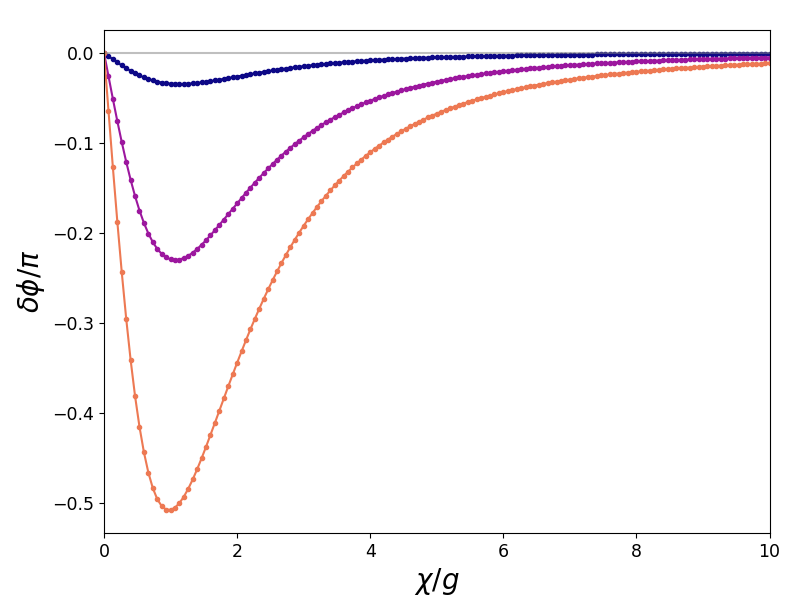
\includegraphics[width=\textwidth]{figuras/ch3/robustez kerr.png}
    \end{minipage}\hfill
    \begin{minipage}[c]{0.3\textwidth}
    \caption{Diferencia de fase geométrica acumulada en función del parámetro del medio $\chi$, para $\Delta=0$ y para 3 medios distintos, cuyas tasas de perdida de fotones son $\gamma/g=0.01g,0.1g,0.25g$, asignadas a los colores violeta oscuro, morado y amarillo respectivamente.
         } \label{fig3:robustez kerr}
  \end{minipage}
\end{figure}
En la figura \ref{fig3:robustez kerr} se observa la dependencia de la diferencia en la fase geométrica acumulada en función del parámetro del medio $\chi$. El comportamiento es el mismo que en el caso anterior, se observa que la diferencia se anula para $\chi=0$, que coincide con el caso de robustez $\Delta=0$. La diferencia es que ahora la fase acumulada es negativa, pero vemos que solo es una reflexión con respecto al caso anterior, esto se debe a que el detunning $\Delta$ y el parámetro del medio $\chi$, tienen signos diferentes en todas las expresiones vistas anteriormente. Esto produce que la fase herede este signo, pero vemos que el comportamiento es el mismo; se observa también que en este caso hay un máximo no trivial que depende suavemente de los parámetros $\gamma/g$ y $p/g$, lo cual nos dice que la dependencia en la fase geométrica en este parámetro no es trivial, y al igual que en el caso del detunning, es no-monótona, por lo tanto tiene las mismas implicancias que en el caso anterior. Lo interesante ahora es intentar de ver como se comportan ambos parámetros en conjunto. Se espera que, por los comportamiento observados hasta ahora, en realidad la dependencia general sea en $\Delta-\chi(2n-1)$, por lo tanto, se realiza nuevamente el estudio de robustez en función del detunning, para un valor $\chi/g=1$, que se observa en la figura \ref{fig3:robustez mixta}.
\begin{figure}[H]
    \begin{minipage}[c]{0.67\textwidth}
        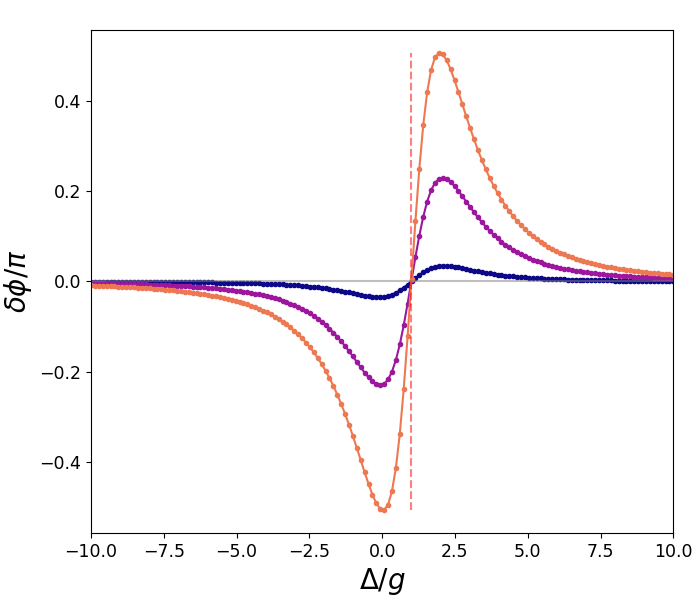
\includegraphics[width=\textwidth]{figuras/ch3/robustez x=g.png}
    \end{minipage}\hfill
    \begin{minipage}[c]{0.3\textwidth}
    \caption{Diferencia de fase geométrica acumulada en función del detunning átomo-cavidad $\Delta$, para $\chi=g$ y para 3 medios distintos, cuyas tasas de perdida de fotones son $\gamma/g=0.01g,0.1g,0.25g$, asignadas a los colores violeta oscuro, morado y amarillo respectivamente. Se observa como la condición de robustez se alcanza para $\Delta/g=\chi/g=1$.
         } \label{fig3:robustez mixta}
  \end{minipage}
\end{figure}
Se observa como ahora tenemos una simetría al rededor de $\Delta=g=\chi$, donde se encuentra el cero de esta relación. Esto es lo que esperábamos, ya que en este caso de $n=1$, esperamos que la dependencia sea en $\Delta-\chi(2n-1) \implies \Delta-\chi$, es decir, si en el caso de $\chi=0$ vimos robustez en el caso resonante $\Delta=0$, lo que esperamos es que los demás casos robustos también se den cuando, en general $\Delta-\chi(2n-1)=0$, comportamiento que se observa en la figura \ref{fig3:robustez mixta}.
\subsubsection{Robustez de la fase geométrica en el caso resonante}

En esta sección se discute la razón detrás de la robustez en los casos estudiados anteriormente. 

Como se ha mencionado, las figuras \ref{fig3:robustez 0}, \ref{fig3:robustez kerr} y \ref{fig3:robustez mixta}, muestran el resultado notable de que la diferencia $\delta\phi$ entre la fase geométrica acumulada en una hipotética evolución unitaria y la fase geométrica acumulada por el sistema abierto se anula cuando se satisface la condición de resonancia $\Delta = 0$. El resultado sugiere que la fase geométrica es robusta a los efectos del entorno en este caso. Esta robustez puede estudiarse y explicarse en términos geométricos analizando la evolución del estado $\rho(t)$ del sistema átomo-modo y se vincula con el salto en $\pi$ que exhibe la fase geométrica unitaria $\phi_u$ del sistema resonante, cuyo estado describe un círculo máximo de la esfera de Bloch.

Para explicar el salto en $\pi$ de la fase unitaria es necesario recordar, como fue desarrollado en las secciones \ref{sec} y \ref{sec}, que la fase geométrica asociada a una trayectoria unitaria no-cíclica puede entenderse como la fase geométrica asociada a una curva cerrada específica: aquella construida a partir de la trayectoria abierta original, luego cerrada mediante una curva geodésica que conecte sus extremos. Esta interpretación permite explicar un salto abrupto en $\pi$ que muestra la fase geométrica acumulada en la evolución del sistema cuando el estado recorre un meridiano de la esfera de Bloch. Debido a que las geodésicas de la esfera de Bloch son, precisamente, sus círculos máximos, cuando la evolución recorre uno de éstos sin alcanzar a transitar la mitad de su longitud, la curva geodésica que debe considerarse coincide con la trayectoria de forma que la curva cerrada retorna sobre si misma acumulando fase geométrica nula. Por el contrario, si la trayectoria descrita por el estado supera la mitad del círculo máximo, la geodésica que une sus extremos lo completa encerrando un área de $2\pi$ que corresponde a una fase geométrica $\phi_u=\pi$.

Para el caso de un sistema en interacción con el entorno, la identidad formal entre la ecuación \ref{ec2}(2.71) y la fase geométrica unitaria para el autoestado $\ket{\psi_+(t)}$ de la matriz densidad demanda el estudio de la curva descrita en la esfera de Bloch por (la proyección de) $\ket{\psi_+(t)}$. Lo que se observa es que para el caso resonante $\ket{\psi_+(t)}$ recorre una trayectoria que se superpone con aquella descrita por su análogo unitario pero que por efecto del entorno resulta de menor longitud (para un intervalo temporal idéntico). En un período $t \in [0, T]$ de evolución, entonces, el rayo asociado al estado $\ket{\psi(t)}$ retorna al punto inicial describiendo una trayectoria cíclica, mientras que aquél asociado a $\ket{\psi_+(t)}$ describe una curva abierta. Sin embargo, esto no afecta el valor obtenido para la fase geométrica que resulta $\phi_g=\pi$ siempre que el rayo recorra más de la mitad del círculo máximo. En consecuencia, siempre y cuando los efectos disipativos no sean lo suficientemente destructivos como para impedir que el autoestado supere el polo opuesto en un intervalo $t' \in [0, T]$, la fase geométrica acumulada en un período no se verá afectada. En este sentido, el caso resonante resulta entonces la situación ideal para realizar detecciones experimentales o implementar aplicaciones tecnológicas que requieran un escenario en que se puedan despreciar los efectos del entorno.